%%%%%%%%%%%%%%%%%%%%%%%%%%%%%%%%%%%%%%%%%
% Article EcoFoG
% Version 2.1 (23/10/2017)
%
% adapté de :
% Stylish Article
% LaTeX Template
% Version 1.0 (31/1/13)
%
% This template has been downloaded from:
% http://www.LaTeXTemplates.com
%
% Original author:
% Mathias Legrand (legrand.mathias@gmail.com)
%
% License:
% CC BY-NC-SA 3.0 (http://creativecommons.org/licenses/by-nc-sa/3.0/)
%
%%%%%%%%%%%%%%%%%%%%%%%%%%%%%%%%%%%%%%%%%


%----------------------------------------------------------------------------------------
%	PACKAGES AND OTHER DOCUMENT CONFIGURATIONS
%----------------------------------------------------------------------------------------

\documentclass[fleqn,10pt]{ArtEcoFoG} % Document font size and equations flushed left

\setcounter{tocdepth}{3} % Show only three levels in the table of contents section: sections, subsections and subsubsections


% Pandoc environments
\usepackage{framed}
\usepackage{fancyvrb}
\providecommand{\tightlist}{%
  \setlength{\itemsep}{0pt}\setlength{\parskip}{0pt}}
\newcommand{\VerbBar}{|}
\newcommand{\VERB}{\Verb[commandchars=\\\{\}]}
\DefineVerbatimEnvironment{Highlighting}{Verbatim}{commandchars=\\\{\}, fontsize=\scriptsize} % Code R
\definecolor{shadecolor}{RGB}{248,248,248}
\newenvironment{Shaded}{\begin{snugshade}}{\end{snugshade}}
\newcommand{\KeywordTok}[1]{\textcolor[rgb]{0.13,0.29,0.53}{\textbf{{#1}}}}
\newcommand{\DataTypeTok}[1]{\textcolor[rgb]{0.13,0.29,0.53}{{#1}}}
\newcommand{\DecValTok}[1]{\textcolor[rgb]{0.00,0.00,0.81}{{#1}}}
\newcommand{\BaseNTok}[1]{\textcolor[rgb]{0.00,0.00,0.81}{{#1}}}
\newcommand{\FloatTok}[1]{\textcolor[rgb]{0.00,0.00,0.81}{{#1}}}
\newcommand{\ConstantTok}[1]{\textcolor[rgb]{0.00,0.00,0.00}{{#1}}}
\newcommand{\CharTok}[1]{\textcolor[rgb]{0.31,0.60,0.02}{{#1}}}
\newcommand{\SpecialCharTok}[1]{\textcolor[rgb]{0.00,0.00,0.00}{{#1}}}
\newcommand{\StringTok}[1]{\textcolor[rgb]{0.31,0.60,0.02}{{#1}}}
\newcommand{\VerbatimStringTok}[1]{\textcolor[rgb]{0.31,0.60,0.02}{{#1}}}
\newcommand{\SpecialStringTok}[1]{\textcolor[rgb]{0.31,0.60,0.02}{{#1}}}
\newcommand{\ImportTok}[1]{{#1}}
\newcommand{\CommentTok}[1]{\textcolor[rgb]{0.56,0.35,0.01}{\textit{{#1}}}}
\newcommand{\DocumentationTok}[1]{\textcolor[rgb]{0.56,0.35,0.01}{\textbf{\textit{{#1}}}}}
\newcommand{\AnnotationTok}[1]{\textcolor[rgb]{0.56,0.35,0.01}{\textbf{\textit{{#1}}}}}
\newcommand{\CommentVarTok}[1]{\textcolor[rgb]{0.56,0.35,0.01}{\textbf{\textit{{#1}}}}}
\newcommand{\OtherTok}[1]{\textcolor[rgb]{0.56,0.35,0.01}{{#1}}}
\newcommand{\FunctionTok}[1]{\textcolor[rgb]{0.00,0.00,0.00}{{#1}}}
\newcommand{\VariableTok}[1]{\textcolor[rgb]{0.00,0.00,0.00}{{#1}}}
\newcommand{\ControlFlowTok}[1]{\textcolor[rgb]{0.13,0.29,0.53}{\textbf{{#1}}}}
\newcommand{\OperatorTok}[1]{\textcolor[rgb]{0.81,0.36,0.00}{\textbf{{#1}}}}
\newcommand{\BuiltInTok}[1]{{#1}}
\newcommand{\ExtensionTok}[1]{{#1}}
\newcommand{\PreprocessorTok}[1]{\textcolor[rgb]{0.56,0.35,0.01}{\textit{{#1}}}}
\newcommand{\AttributeTok}[1]{\textcolor[rgb]{0.77,0.63,0.00}{{#1}}}
\newcommand{\RegionMarkerTok}[1]{{#1}}
\newcommand{\InformationTok}[1]{\textcolor[rgb]{0.56,0.35,0.01}{\textbf{\textit{{#1}}}}}
\newcommand{\WarningTok}[1]{\textcolor[rgb]{0.56,0.35,0.01}{\textbf{\textit{{#1}}}}}
\newcommand{\AlertTok}[1]{\textcolor[rgb]{0.94,0.16,0.16}{{#1}}}
\newcommand{\ErrorTok}[1]{\textcolor[rgb]{0.64,0.00,0.00}{\textbf{{#1}}}}
\newcommand{\NormalTok}[1]{{#1}}
\usepackage{longtable,booktabs}
\usepackage{caption}
% These lines are needed to make table captions work with longtable:
\makeatletter
\def\fnum@table{\tablename~\thetable}
\makeatother
% longtable 2 columns
% https://tex.stackexchange.com/questions/161431/how-to-solve-longtable-is-not-in-1-column-mode-error
\makeatletter
\let\oldlt\longtable
\let\endoldlt\endlongtable
\def\longtable{\@ifnextchar[\longtable@i \longtable@ii}
\def\longtable@i[#1]{\begin{figure}[t]
\onecolumn
\begin{minipage}{0.5\textwidth}\scriptsize
\oldlt[#1]
}
\def\longtable@ii{\begin{figure}[t]
\onecolumn
\begin{minipage}{0.5\textwidth}\scriptsize
\oldlt
}
\def\endlongtable{\endoldlt
\end{minipage}
\twocolumn
\end{figure}}
\makeatother

\usepackage{graphicx,grffile}
\makeatletter
\def\maxwidth{\ifdim\Gin@nat@width>\linewidth\linewidth\else\Gin@nat@width\fi}
\def\maxheight{\ifdim\Gin@nat@height>\textheight0.8\textheight\else\Gin@nat@height\fi}
\makeatother
% Scale images if necessary, so that they will not overflow the page
% margins by default, and it is still possible to overwrite the defaults
% using explicit options in \includegraphics[width, height, ...]{}
\setkeys{Gin}{width=\maxwidth,height=\maxheight,keepaspectratio}

% User-adder preamble
\usepackage{textcomp} \DeclareUnicodeCharacter{B0}{\textdegree}
\usepackage{tabu} \usepackage{caption}
\captionsetup{justification = justified}
\renewenvironment{table}{\begin{table*}}{\end{table*}\ignorespacesafterend}
\hyphenation{bio-di-ver-si-ty sap-lings}

%----------------------------------------------------------------------------------------
%	ARTICLE INFORMATION
%----------------------------------------------------------------------------------------

\JournalInfo{Hal xxx} % Journal information
\Archive{DOI xxxx} % Additional notes (e.g. copyright, DOI, review/research article)

\PaperTitle{Post-Disturbance Tree Community Trajectories in a Neotropical Forest} % Article title

\Authors{
Ariane MIRABEL\textsuperscript{1*}\\ Eric Marcon\textsuperscript{1}\\ Bruno Hérault\textsuperscript{2 3}
} % Authors
\affiliation{
\textsuperscript{1}UMR EcoFoG, AgroParistech, CNRS, Cirad, INRA, Université des Antilles,
Université de Guyane.\\ \hspace{1em} Campus Agronomique, 97310 Kourou, France.\\\textsuperscript{2}Cirad, Univ montpellier, UR Forests \& Societies.\\ \hspace{1em} Montpellier, France.\\\textsuperscript{3}INPHB, Institut National Polytechnique Félix Houphouet-Boigny\\ \hspace{1em} Yamoussoukro, Ivory Coast.
}
\affiliation{*\textbf{Corresponding author}: ariane.mirabel@ecofog.gf, http://www.ecofog.gf/spip.php?article47} % Corresponding author

\Keywords{Taxonomic and Functional Biodiversity, Neotropical Forests, Disturbance Trajectories, Intermediate Disturbance Hypothesis, Long-term Resilience} % Keywords - if you don't want any simply remove all the text between the curly brackets
\newcommand{\keywordname}{Keywords} % Defines the keywords heading name

%----------------------------------------------------------------------------------------
%	ABSTRACT
%----------------------------------------------------------------------------------------

\Abstract{
Understand the maintenance of forests biodiversity structure,
functioning and dynamics is urgent to anticipate their fate in the
global changing context. Communities diversity structure is assumed to
rely on a constant regime of disturbance and peak at intermediate
intensity. For tropical forests this intermediate disturbance hypothesis
(IDH) remain debated as well as the completeness of forests resilience
in all taxonomic and functoinal facets. To disentangle the ecological
processes driving forests dynamics we examined the the trajectories over
30 years after a gradient of logging and thinning disturbance, focusing
on communities taxonomic and functional composition and diversity.
Specifically we analysed the trajectories of communities taxonomic
richness and evennes and functional composition, diversity and
redundancy based on 7 key functional traits assessing species ecology.
We highlighted a decoupling between functional and taxonomic
trajectories, translating a fast recovery of communities functioning
while their taxonomic recovery was slowed by the recruitment of
infrequent species specific to mature forests. The IDH consistently
predicted communities functional trajectories but poorly reflected the
taxonomic ones, blurried by changes in the functional redundancy
entailing competitive exclusion. Although communities consistently
recovered their functioning after 30 years, initially infrequent species
proved long to recover which impacted the taxonomic structure and
functoinal redundancy over several decades. Our results acknowledged the
need of decades-long recovery cycles to restore the resilience of the
community and prevent species loss in the long term.
}

%----------------------------------------------------------------------------------------

\usepackage{amsthm}
\newtheorem{theorem}{Theorem}[section]
\newtheorem{lemma}{Lemma}[section]
\theoremstyle{definition}
\newtheorem{definition}{Definition}[section]
\newtheorem{corollary}{Corollary}[section]
\newtheorem{proposition}{Proposition}[section]
\theoremstyle{definition}
\newtheorem{example}{Example}[section]
\theoremstyle{definition}
\newtheorem{exercise}{Exercise}[section]
\theoremstyle{remark}
\newtheorem*{remark}{Remark}
\newtheorem*{solution}{Solution}
\begin{document}

\selectlanguage{english}

\flushbottom % Makes all text pages the same height

\maketitle % Print the title and abstract box

\tableofcontents % Print the contents section

\thispagestyle{empty} % Removes page numbering from the first page

%----------------------------------------------------------------------------------------
%	ARTICLE CONTENTS
%----------------------------------------------------------------------------------------
























\section{Introduction}\label{introduction}

The large areas covered with tropical forests worldwide hold crucial
environmental, economic and social values. They provide wood and
multiple non-timber forest products, shelter a diversified fauna,
regulate the local climate, support the carbon, water and nutrient
cycles, and ensure cultural and human well-being. The simultaneous
increased demand in forests products and the substantial climatic
changes currently heighten the pressure on remaining forests
\citep{Gibson2011a, Morales-Hidalgo2015}, threatening the maintenance of
communities structure, composition and functioning and their dynamics in
space and time \citep{Anderson-Teixeira2013, Sist2015}.

In tropical forest, ecological communities are constantly re-shaped by
natural disturbance events that change both abiotic environment, through
the fluxes of light, heat and water \citep{Goulamoussene2017}, and
biotic interactions like competition among species \citep{Herault2018}.
The cornerstone of tropical forests ecology is to understand the
mechanisms and the determinants of ecosystems response to disturbance
\citep{White2001, Chazdon2003a}. For now, this has been largely studied
through structural parameters, rapid and convenient to measure, as
aboveground biomass, tree height or stem density
\citep{Piponiot2016, Rutishauser2016}. These structural parameters were
thereafter sucessfully modeled, giving important insights into the
maintenance of ecosystems processes and services
\citep{Denslow2000, Blanc2009}. However the response of forests
diversity in tree species remains unclear, albeit it determines the
productivity, stability and functioning of ecosystems
\citep[\citet{Liang2016}]{Tilman2014} and would be most probably
impacted by the changes following disturbance \citep{Baraloto2012a}.

In the short-term disturbance demonstrated negligible or even positive
impacts on communities diversity, which have been formalized by the
intermediate disturbance hypothesis (IDH) stating a maximized species
diversity at intermediate disturbance intensity
\citep{Molino2001, Kariuki2006a, Berry2008a}. Still, validations of the
IDH remain scarce in the long term and mainly rely on species richness
analyses that give limited or misleading information on forests recovery
and functioning \citep{Martin2015, Chaudhary2016}. More releveant
monitoring would encompass communities composition, crucial for
conservation issues, and complete diversity profiles integrating both
species richness and evenness, to reveal the ecological rules
structuring communities \citep{Magurran1988, Lavorel2002, Bellwood2006}.
Furthermore, the functional approach that accounts for species
biological attributes and role in the ecosystem would be essential to
understand the correlations between ecosystems biodiversity, functioning
and environmental constraints
\citep{Violle2007b, Moretti2009, Baraloto2012a, Scheiter2013}. The
functional trait-based approach focused on major traits related to
species ecology and performance was sucessfully adopted
\citep{Diaz2005, Villeger2008a}, for example in highlighting
deterministic processes in tropical rainforests that foster fast growing
species with efficient resources acquisition after disturbance
\citep{Molino2001, Haddad2008, Ruger2009}. Communities then shifted from
a dominance of ``conservative'' slow-growing species dealing with scarce
resources to ``acquisitive'' fast-growing species with rapid and
efficient use of abundant resources
\citep{TerSteege2001, Reich2014, Herault2011}. This shift translated
into consistent trajectories for key functional traits related to
resource acquisition (leaf area, density and chlorophyll content, and
stem specific gravity and bark thickness), tree growth and reproduction
and life history traits (seed mass and maximum height)
\citep{Wright2004, Westoby2006a, Chave2009b}.

A combination of taxonomic and functional approaches are essential to
fully assess communities response to disturbance and differences in
their respective trajectories are insightful of underlying mechanisms
\citep{Lohbeck2015, Guariguata2001}. Although taxonomic and functional
diversity are complementary and sometimes decouples, they are combined
in the measure of communities functional redundancy that quantifies the
amount of shared trait values among species \citep{Carmona2016}.
Functional redundancy is determinant of communities resilience as high
redundancy, like in highly diverse tropical forests
\citep{Bellwood2006}, mitigates the impacts of species removal on
ecosystem functioning \citep{Trenbath1999, Elmqvist2003, Diaz2005}.

Grasp all facets of communities response to disturbance comes to examine
the taxonomic and functional trajectories in diversity and composition.
These trajectories would highlight the ecological rules constraining or
not communities dynamics towards the recovery of initial composition,
diversity and functioning. They would therefore clarify the tenants in
the long term of the debated Intermediate Disturbance Hypothesis for
tropical forests, a cruicial point for future adaptive conservation
strategies \citep{Adler2007}. Here we monitored over 30 years the
response of 75 ha of forests plots set up on a gradient of disturbance
intensity, from 10 to 60\% of ecosystem biomass removed. We made use of
a large functional traits database browsing major leaf, stem and seed
functional traits and species maximum height to draw the trajectories
over time of communities taxonomic and functional composition and
diversity. Specifically, we (i) questioned the coupling between
taxonomic and functional response to disturbance and identified the
underlying assembly processes, which allowed to (ii) clarify the
validity of the IDH in the long term for tropical forest and (iii)
question the completeness of communities recovery regarding their
functional redundancy.

\section{Material and Methods}\label{material-and-methods}

\subsection{Study site}\label{study-site}

Paracou station in French Guiana (5°18'N and 52°53'W) is located in a
lowland tropical rain forest in a tropical wet climate with mean annual
temperature of 26°C, mean annual precipitation averaging 2980
mm.y\textsuperscript{-1} (30-y period) and a 3-month dry season
(\textless{} 100 mm.month\textsuperscript{-1}) from mid-August to
mid-November, and a one-month dry season in March \citep{Wagner2011}.
Elevation ranges between 5 and 50 m and soils correspond to thin
acrisols over a layer of transformed saprolite with low permeability
generating lateral drainage during heavy rains.

The experiment is a network of twelve 6.25ha plots that underwent a
gradient of three logging, thinning and fuelwood cutting treatments
(Table \ref{tab:Tab1}). Disturbance treatments were attributed according
to a randomized plot design with three replicate blocks of four plots.
The disturbance corresponds to averages of 10 trees removed per hectare
with a diameter at 1.3 m height (DBH) above 50 cm for treatment 1 (T1),
32 trees/ha above 40 cm DBH for treatment 2 (T2) and 40 trees/ha above
40 cm DBH for treatment 3 (T3). Treatments T2 and T3 besides included
the thinning of trees by poison girdling \citep{Schmitt1989, Blanc2009}.
The disturbance intensity was measured as the percentage of aboveground
biomass (\%AGB) lost between the first inventory in 1984 and five years
after disturbance (ref to be found) measured with the BIOMASS R package
\citep{Biomass2018}.

\begin{table}

\caption{\label{tab:Tab1}Intervention table, summary of the disturbance intensity for the 4 plot treatments in Paracou.}
\centering
\begin{tabu} to \linewidth {>{\raggedright}X>{\raggedright}X>{\raggedright}X>{\raggedright}X>{\raggedright}X}
\toprule
Treatment & Timber & Thinning & Fuelwood & \%AGB lost\\
\midrule
Control &  &  &  & 0\\
T1 & DBH $\geq$ 50 cm, commercial species, $\approx$ 10 trees/ha &  &  & $[12\%-33\%]$\\
T2 & DBH $\geq$ 50 cm, commercial species, $\approx$ 10 trees/ha & DBH $\geq$ 40 cm, non-valuable species, $\approx$ 30 trees/ha &  & $[33\%-56\%]$\\
T3 & DBH $\geq$ 50 cm, commercial species, $\approx$ 10 trees/ha & DBH $\geq$ 50 cm, non-valuable species, $\approx$ 15 trees/ha & 40 cm $\leq$ DBH $\leq$ 50 cm, non-valuable species, $\approx$ 15 trees/ha & $[35\%-66\%]$\\
\bottomrule
\end{tabu}
\end{table}

\subsection{Inventories protocol and dataset
collection}\label{protocols}

The study site corresponds to a tropical rainforest with a dominance of
Fabaceae, Chrysobalanaceae, Lecythidaceae and Sapotaceae botanical
families. In the twelve experimental plots of the experiment, all trees
above 10 cm DBH are mapped and measured annually since 1984. Trees are
first identified during inventories with a vernacular name assigned by
the field team, and afterward with a scientific name assigned by a
botanist during regular botanical campaigns. In 1984, specific
vernacular names are given to 62 commercial or common species whereas
more infrequent ones were identified under general identifiers only
distinguiching trees and palm trees. From 2003 botanical campaigns were
conducted every 5 to 6 years to identify all trees at the species level
but identification practices still varied among plots and campaigns.

This variability of protocols raised methodological issues as vernacular
names usually correspond to different botanical species. It resulted in
significant taxonomic uncertainties that had to be propagated to
composition and diversity metrics. The uncertainty propagation was done
through a Bayesian framework reconstituting complete inventories at
genus level from real incomplete ones on the basis of
vernacular/botanical names association. Vernacular names were replaced
through multinomial trials
\(M_v\Big(\big[s_1, s_2, …, s_N\big],\big[\alpha_1, \alpha_2,…, \alpha_3\big]\Big)\)
based on the association probability
\(\big[\alpha_1, \alpha_2,…, \alpha_3\big]\) observed across all
inventories between each vernacular name \emph{v} and the species
\(\big[s_1, s_2, …, s_N\big]\). See appendix 1 and
\citet{Aubry-Kientz2013} for the detailed methodology.

The functional approach used a dataset of 6 functional traits
representing leaf economics (leaves thickness, toughness, total
chlorophyll content and specific leaf area, the leaf area per unit dry
mass) and wood economics (wood specific gravity and bark thickness), and
life history traits (maximum specific height and seed mass). The trait
database came from the BRIDGE project \footnote{http://www.ecofog.gf/Bridge/}
where trait values were assessed from a selection of individuals located
in nine permanent plots in French Guiana, including two in Paracou, and
comprised 294 botanical species pertaining to 157 botanical genera.
Missing trait values were filled using multivariate imputation by
chained equation (mice) from the mice R package \citep{Mice2011}.
Imputations were restricted within genus, or family when samples wre too
scarce, in order to account for the phylogenetic signal of the
functional traits. Whenever a species inventoried was not in the
dataset, it was attributed a set of traits values randomly sampled among
species of the same next higher taxonomic level (same genus or family).
As seed mass information corresponds to a classification into mass
classes, no data filling process was applied and analysis were
restricted to the 414 botanical species recorded.

All composition and diversity metrics corresponded to the average
obtained after 50 iterations of the taxonomic uncertainty propagation
framework and of the filling process of missing trait values.

\subsection{Composition and diversity
metrics}\label{composition-and-diversity-metrics}

To counter taxonomic uncertainties due to the variability of botanical
identification protocols (see {[}\#protocols{]}), the taxonomic
composition and diversity analysis were conducted at the genus level,
\emph{i.e.} referring to the genus of observed or trialed botanical
names. Trajectories of communities taxonomic and functional variations
in composition after disturbance were followed in a two-dimensional
ordination space the 30 years monitored. Two NMDS were conducted to map
either taxonomic flora inventories or communities functional composition
based on the 7 leaf, stem and life history traits (without seed mass
classes). In both cases the NMDS were performed using occurrence-based
(Jaccard) and abundance-based (Bray-Curtis) dissimilarity measures.
Trajectories along time in the plan were reported through the euclidean
distance of successive inventories to the reference inventories in 1989,
5 years after disturbance, when the uncertainty degree did not exceed
30\% of undetermined trees. The trajectories of the leaf and stem and
life traits were also visualized with the community weighted means
(CWM), representing the average trait value in a community weighted by
relative abundance of the species carrying each value
\citep{Diaz2007, Garnier2004}. To compensate the intrinsinc difference
among plots the trajectories corresponded to the differences along time
with the reference inventory in 1989. Species seed mass corresponded to
5 classes of increasing mass, seed mass trajectories were therefore
reported as the proportion of each class in the inventories.

The taxonomic diversity was assessed through Richness and the Hill
number translation of Shannon and Simpson indices \citep{Hill1973}.
These three indices belong to the set of HCDT or generalized entropy,
respectively corresponding to the 0, 1 and 2 order of diversity (q),
recomended for diversity studies \citep{Patil1982, Tothmeresz1995}. The
functional diversity was reported using the Rao index of quadratic
entropy which combines species abundance distribution and average
pairwise dissimilarity based on all functional and life traits.

The impacts of initial disturbance were first tested with the spearman
rank correlation between the extremum of taxonomic and functional
metrics reached over the 30 years and the initial \%AGB removed. Then
they were analysed through the linear correlations between Simpson and
Rao diversities and the initial \%AGB removed at 10, 20 and 30 years
after disturbance.

The functional redundancy was measured as the overlap among species in
communities' functional space \citep{Carmona2016}. The samples of the
trait database were first mapped in a 2-dimensional plan from a PCA
analysis. Then, multivariate kernel density estimator associated with
individual trees returned species traits probability distribution (TDP).
Species TDP weighted by species abundance were eventually summed for
each community: the functional redundancy was the sum of TDPs overlap,
expressed as the average number of species that could be removed from
without reducing the functional space (see appendix I for a more
comprehensive sheme).

\section{Results}\label{results}

\subsection{Communities Diversity}\label{communities-diversity}

In the inventories from 1989 (5 years after disturbance) to 2015 (31
years after disturbance), 828388 trees and 591 botanical species
pertaining to 223 genus and 64 botanical families were recorded.
Communities taxonomic diversity trajectories were examined through the
Richness, Shannon and Simpson diversities at genus level, in relation to
the 1989 inventories (5 years after disturbance) (See annexe I). For
undisturbed plots the Richness, Shannon and Simpson diversities remained
stable over the 30 years monitored. In disturbed communities the
taxonomic richness increased after low disturbance intensity, reaching a
maximum gain of 14 botanical genera (plot 3 from treatment 2) while it
followed unimodal trajectories after intense disturbance, decreasing for
ten years before recovering pre-disturbance values. In all disturbed
plots the taxonomic evenness (Shannon and Simpson diversities)
increased, following unimodal trajectories with a maximum, reached after
around 20 years, positively correlated to the disturbance treatment
(\(\rho_{spearman}^{Shannon}=0.86\), and
\(\rho_{spearman}^{Simpson}=0.89\)). Return towards initial evenness
values was beginning after 30 years except for two T3 plots (plots 8 and
12) which evenness still increased, suggesting similar but delayed
trajectories \ref{fig:IDHplot}.

Trajectories of communities functional diversity were examined through
the Rao diversity based on the 7 leaf, stem and life history traits (to
the exception of seed mass). The plot 7 from treatment 1 displayed a
constantly outlying diversity and was removed from the graphical
representation for better readability (see appendix for full graphs). In
undisturbed plots the functional diversity remained stable along the 30
years while in disturbed plots it followed unimodal trajectories with a
return towards initial values that strated around 20 years after
disturbance.

The impact of disturbance was examined specifically through the linear
correlation between the intial \%AGB removed and the Simpson and Rao
diversities (diversities of order 2) after 10, 20 and 30 years
\ref{fig:IDHplot}. The correlation with disturbance intensity was weak
for the Simpson diversity (\(R^2<0.25\)) and only valid from 20 years
after disturbance but it was much stronger for the Rao diversity
(\(0.60<R^2<0.75\)) for all the time studied. Slope of linear
correlations, reflecting the impact of disturbance, was the highest 20
years after disturbance.

\begin{figure*}

{\centering 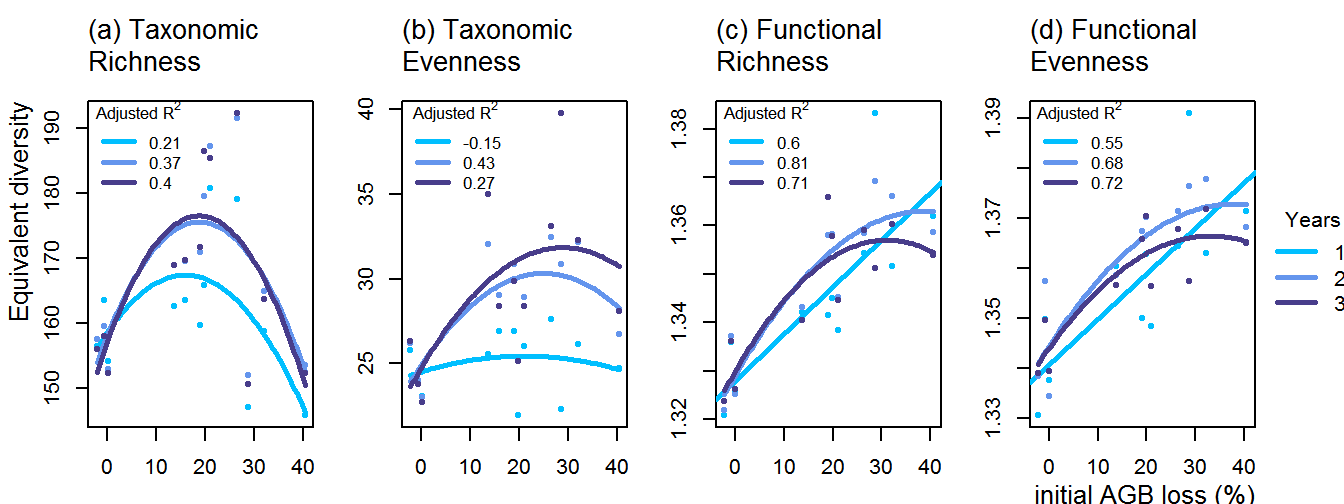
\includegraphics[width=1\linewidth]{WholePlotTrajectories_files/figure-latex/IDHplot-1} 

}

\caption{Upper panels, Trajectories of the Simpson taxonomic diversity \textbf{(a)} and Rao functional diversity \textbf{(b)} over 30 years after disturbance, corresponding to the median and 0.025 and 0.975 percentile observed after 50 iteration of the taxonomic uncertainty propagation and the missing trait value filling processes. Initial treatments are represented by solid lines colors with green for control, blue for T1,orange for T2 and red for T3. Lower panels, Relationship between the initial \%AGB removed and the median values of Simpson \textbf{(c)} and Rao \textbf{(d)} diversities at three times after disturbance. Solid lines colors represent the time, 10 years (yellow), 20 years (orange) and 30 years (brown) after disturbance.}\label{fig:IDHplot}
\end{figure*}

\subsection{Communities composition}\label{communities-composition}

\subsubsection{Taxonomic and functional
trajectories}\label{taxonomic-and-functional-trajectories}

The trajectories of taxonomic and functional composition were visualized
in a two dimensional ordination space mapping the successive inventories
according to their flora and corresponding traits. Classifications were
performed using either abundance-based Bray-Curtis (Figure
\ref{fig:NMDSplans}) or incidence-based Jaccard dissimilarity, both
giving similar results only analysis using Bray-Curtis dissimilarity are
discussed.

While both taxonomic and functional composition remained stable in
undistrubed communities, they followed consistent trajectories over time
after disturbance which revealed significant compositional changes.
According to the mapping of functional traits (see appendix I) these
compositional changes corresponded to shifts towards species with more
acquisitive functional strategies, from communities with high average WD
to high average SLA and chlorophyll content. For disturbed communities
the distance of successive inventories to the 1989 reference inventory
followed unimodal trajectories translating cyclic compositional changes
with a recovery of the initial composition (Figure \ref{fig:NMDSplans}).
The maximum dissimilarity with the initial state was positively
correlated to the disturbance treatment for both taxonomic and
functional composition (\(\rho_{spearman}^{taxonomic}=0.91\) and
\(\rho_{spearman}^{functional}=0.96\) respectively) and the time at
maximum was reached around 26 years after disturbance for taxonomic
composition and 22 years for functional composition.

\begin{figure*}

{\centering 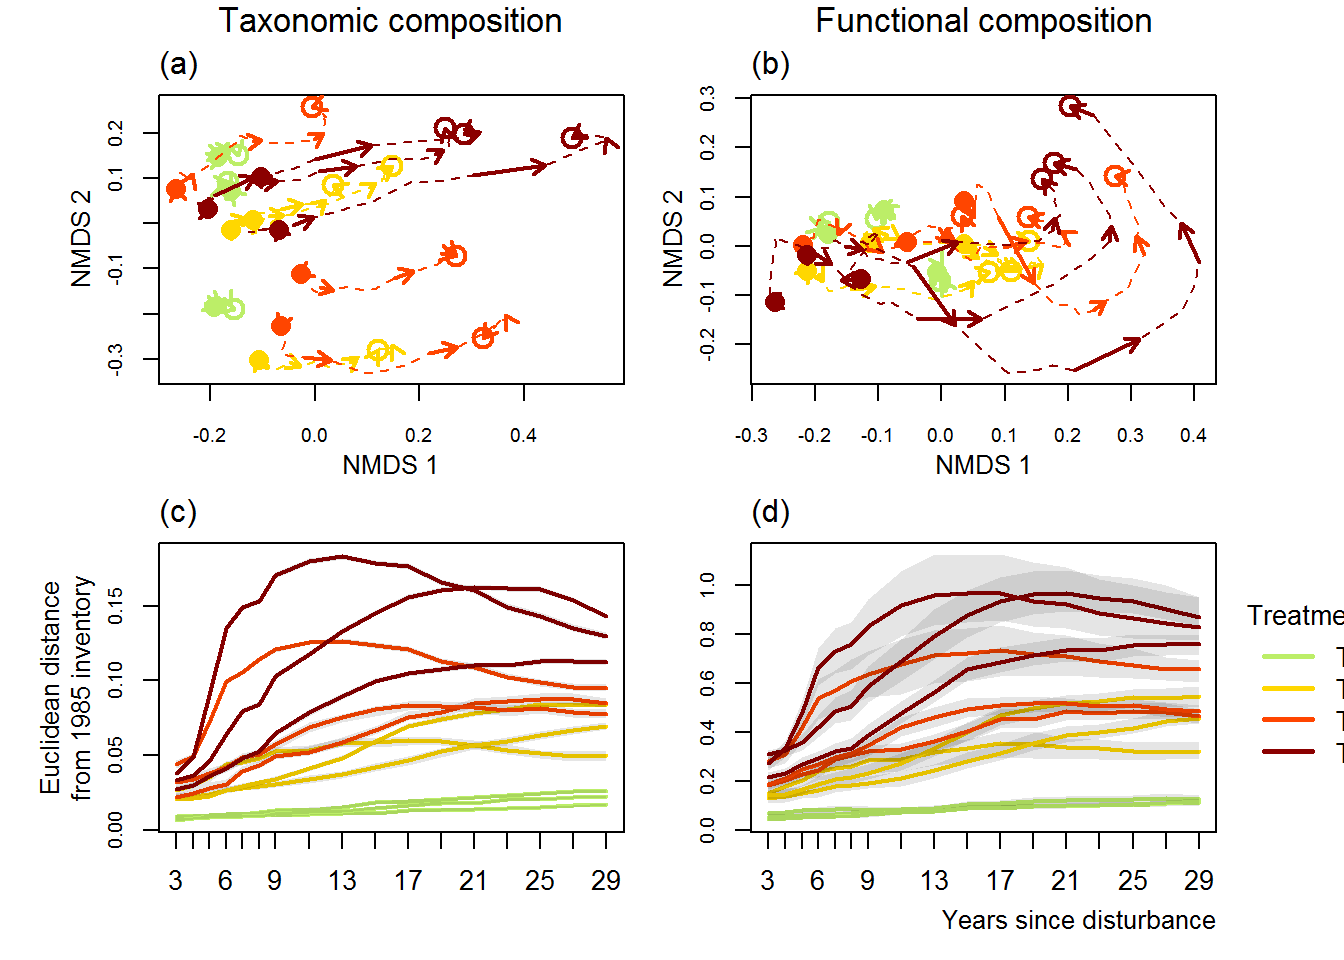
\includegraphics[width=1\linewidth]{WholePlotTrajectories_files/figure-latex/NMDSplans-1} 

}

\caption{Trajectories of the plots in terms of flora composition (left panels \textbf{(a)} and \textbf{(c)}) and functional composition (right panels \textbf{(b)} and \textbf{(d)}) regarding the 6 leaf and stem functional traits, the maximum allometric height and seed mass class. Plots trajectories are first represented in the two-dimensional space from the NMDS performed for the 30 years after disturbance based on Bray-Curtis dissimilarity measures between successive inventories (Upper panels \textbf{(a)} and \textbf{(b)}). Then the lower panels (\textbf{(c)} and \textbf{(d)}) represent the euclidean distance to initial condition along the 30 sampled years. Line colors represent the disturbance treatment (green for control, blue for T1,orange for T2 and red for T3). The 0.025 and 0.975 percentile correspond to the variance observed for 50 iteration of the taxonomic uncertainty propagation and functional trait filling processes.}\label{fig:NMDSplans}
\end{figure*}

\subsubsection{Traits community weighted means
(CWM)}\label{traits-community-weighted-means-cwm}

The changes observed in plots functional composition went hand to hand
with consistent trajectories of the 8 functional and life history traits
visualized with the trajectories of community weighted means (CWM) of
leaves economics (leaves thickness, chlorophyll content, toughness and
specific area), wood economics (wood specific gravity, bark thickness),
and life history traits (seed mass and maximum adult height) (Figure
\ref{fig:CWM}).

Except for leaf chlorophyll content, which continued to increase for
some T3 and T2 plots 30 years after disturbance, all traits and seed
mass proportions followed unimodal trajectories either stabilizing or
returning towards their initial values. Thirty years after disturbance
the weighted means of communities specific maximum height at adult stage
(\emph{Hmax}), leaf toughness (\emph{L\_toughness}) and wood specific
gravity (\emph{WD}) remained significantly lower than their initial
value (Figure \ref{fig:CWM}). The weighted means of bark thickness
(\emph{Bark\_thick}) similarly remained substantially higher than
initially for all disturbed plots while the specfic leaf area
(\emph{SLA}) had almost recovered its initial value. For all traits the
maximum difference to initial state was correlated to the disturbance
intensity (\(\rho_{spearman}^{L_{thickness}}=0.67\),
\(\rho_{spearman}^{L_{chloro}}=0.45\),
\(\rho_{spearman}^{L_{toughness}}=-0.43\),
\(\rho_{spearman}^{SLA}=0.93\), \(\rho_{spearman}^{WD}=-0.78\),
\(\rho_{spearman}^{Bark-thickness}=0.88\),
\(\rho_{spearman}^{Hmax}=-0.48\)).

\begin{figure*}

{\centering 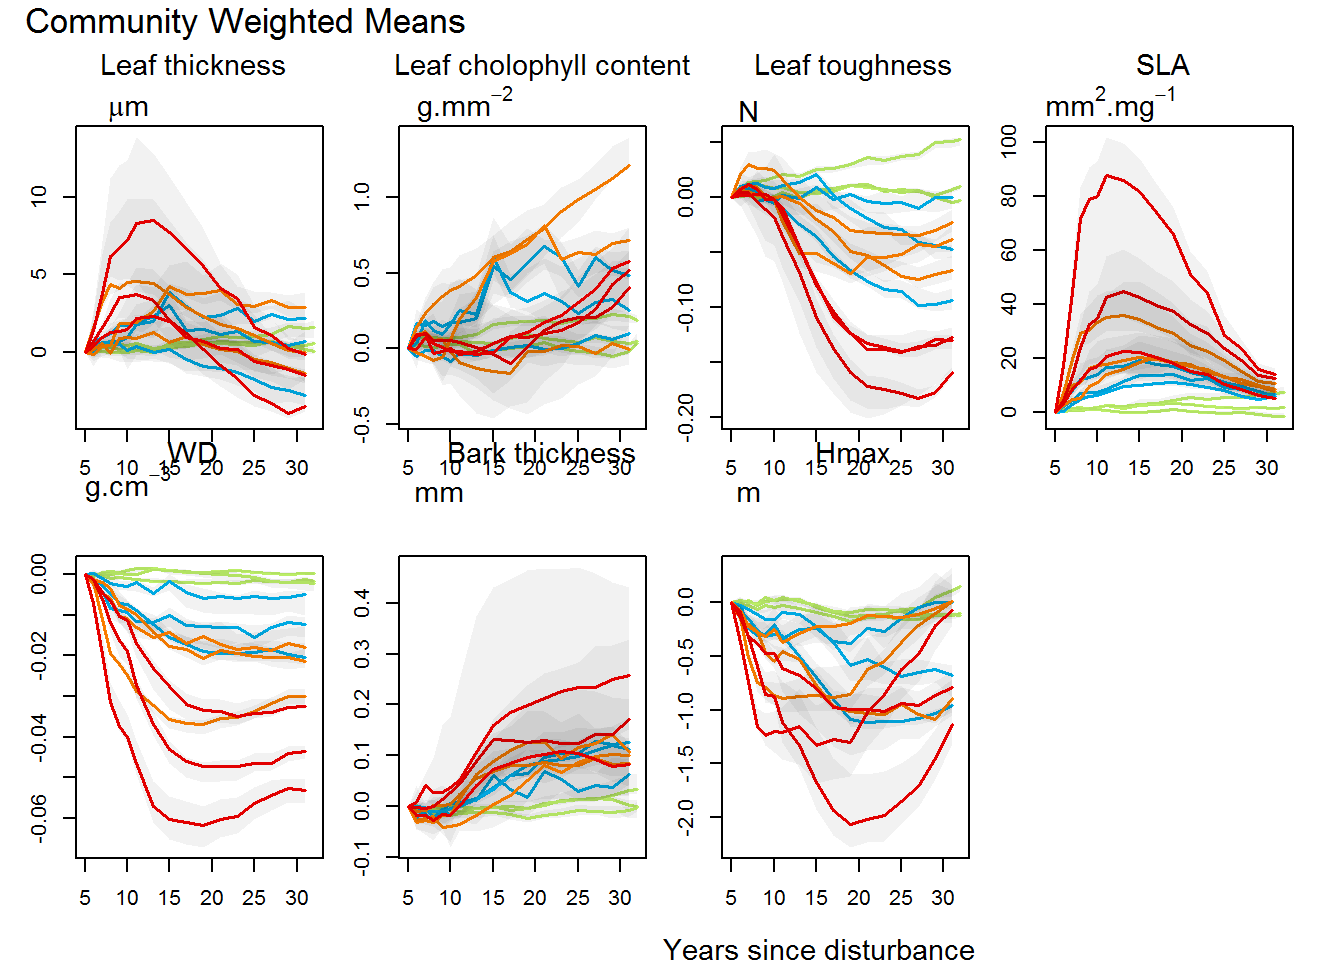
\includegraphics[width=1\linewidth]{WholePlotTrajectories_files/figure-latex/CWM-1} 

}

\caption{Trajectories of the communities weighted means (CWM) over 30 years after disturbance of 4 leaf traits (Leaf thickness, \emph{L\_thickness}, chlorophyll content, \emph{L\_chloro}, toughness, \emph{L\_toughness} and specific area, \emph{SLA}), 2 stem traits (wood specific gravity, \emph{WD}, and bark thickness, \emph{Bark-thick}) and one life trait (Specific maximum height at adult stage, \emph{Hmax}). Trajectories correspond to the median (solid line) and 0.025 and 0.975 percentile (gray envelope) observed after 50 iteration of the taxonomic uncertainty propagation and the missing trait value filling processes. Initial treatments are represented by solid lines colors with green for control, blue for T1,orange for T2 and red for T3.}\label{fig:CWM}
\end{figure*}

\subsubsection{Functional redundancy}\label{functional-redundancy}

Communities functional redundancy was measured as the sum within
communities the species weighted functional overlap based on the 7 leaf,
stem, and maximum height traits (see appendix I for PCA details).
Communities functional redundancy remained stable in control plots but
after disturbance the redundancy trajectories were quite variable (See
appendix I) and apparently independently of the initial disturbance.
Globally after most intense disturbance (plots T2 and T3) communities
redundancy decreased at first place before increasing to edge, recover
or exceed the initial value.

Considering the functional redundancy restricted to the functional space
of the initial inventory, all disturbed plots followed similar
decreasing humped shaped trajectories (@ref(fig:RedFun\_rest)). The
maximum redundancy loss was positively correlated with the disturbance
intensity (XX spearman to be measured) and the initial value had not
recovered for any disturbed communities.

\begin{figure}

{\centering 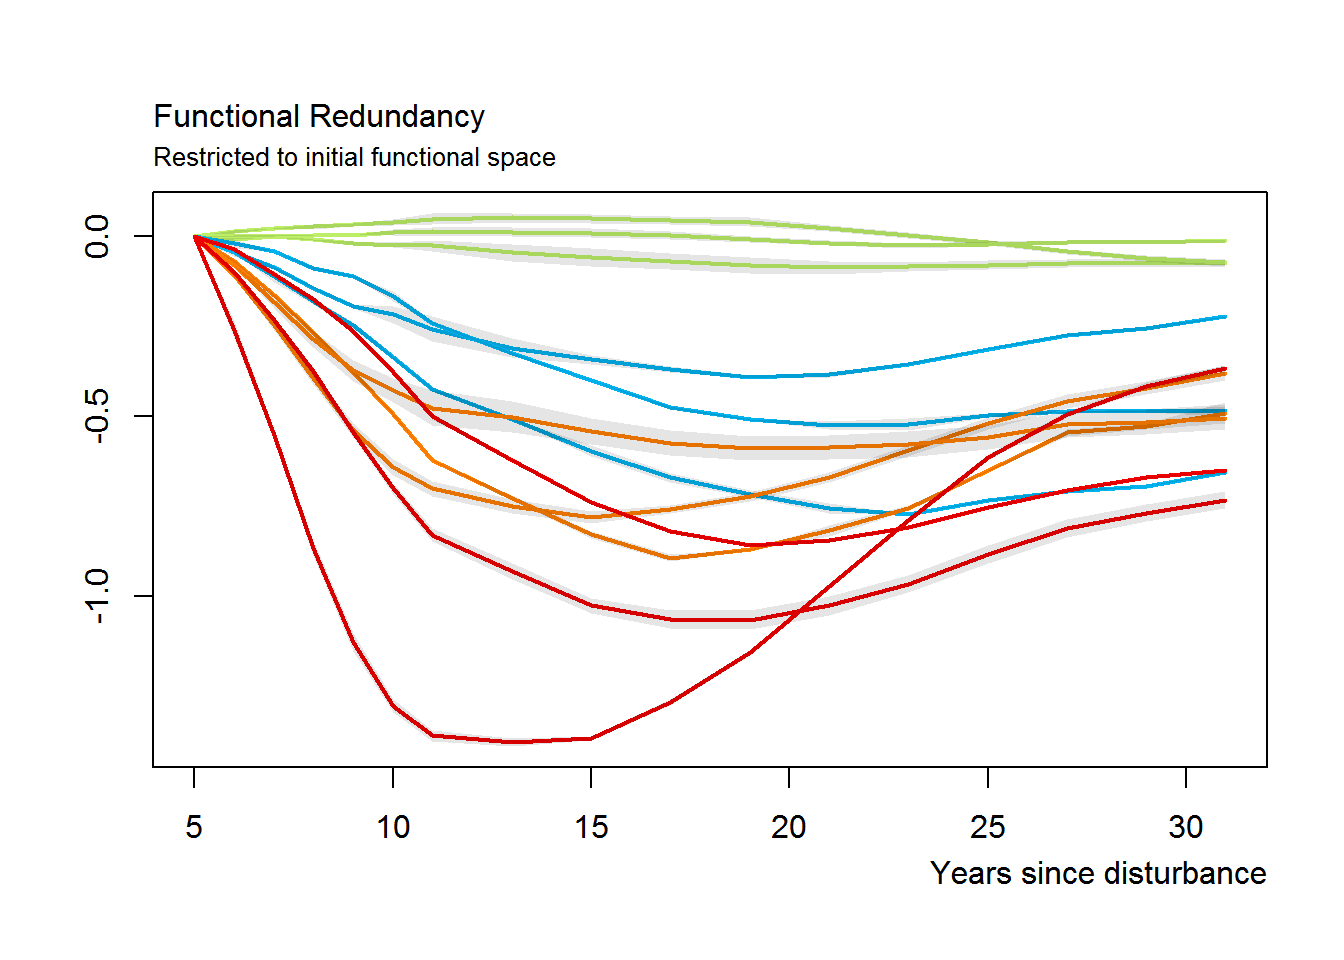
\includegraphics[width=1\linewidth]{WholePlotTrajectories_files/figure-latex/RedFun_rest-1} 

}

\caption{Trajectories of the functional redundancy within the initial cpùùunities functional space over 30 years after disturbance. Trajectories correspond to the median (solid line) and 0.025 and 0.975 percentile (gray envelope) observed after 50 iteration of the taxonomic uncertainty propagation and the missing trait value filling processes. Initial treatments are represented by solid lines colors with green for control, blue for T1,orange for T2 and red for T3.}(\#fig:RedFun_rest)
\end{figure}

\section{Discussion}\label{discussion}

\subsection{Decoupled taxonomic and functional
trajectories}\label{decoupled-taxonomic-and-functional-trajectories}

Both communities taxonomic and functional diversity and composition
proved resilient, following similar humped shaped trajectories returning
towards initial values. The resilience of communities functional
structure, that is the most direct link between biodiversity and
ecosystem functioning \citep{Diaz2005}, meant a consistent recovery of
ecosystem processes in the long term \citep{Guariguata2001}. The
resilience of communities taxonomy meant the maintenance of their
initial differences in composition and diversity, suggesting the
existence of multiple stable equilibria as assumed for highly diverse
and productive ecosystems \citep{Chase2003}, and the dependency of
recovery trajectories on the initial composition to be recovered that
would the the asymptot of the humped shaped dynamics
\citep{Hubbell1999, Molino2001, Anderson2007, Baraloto2012a}.

Although both communities taxonomic and functional characteristics
proved resilient and followed similar humped shaped trajectories, the
taxonomic recovery systematically lagged behind the functional one. The
decoupling between functional and taxonomic dynamics has already been
observed for grasslands \citep{Tilman1997, Mouillot2011} and more
recently for tropical forests \citep{Lohbeck2015, Guariguata2001}.
According to the ``vegetation quantity effect'' \citep{Grime1998}
functional trajectories rely on the pool of dominant species, which
diversity and evenness increased after disturbance but rapidly recovered
their initial functional structure. Although the pool of dominant
species recovered quickly, communities evenness remained high so
infrequent species still missed to the taxonomic recovery. Taxonomic
recovery was then all the more longer that unrecovered species would be
functionally redundant and probably underwent selective competition
processes.

\subsection{A validation of the intermediate disturbance
hypothesis}\label{a-validation-of-the-intermediate-disturbance-hypothesis}

In accordance with the IDH the trajectories confirmed the increase of
communities diversity after disturbance with the favored growth of
otherwise less favored species. However, although it was clear for the
functional diversity this tendency was more blurry regarding communities
taxonomic structure.

The taxonomic richness was enhanced after low disturbance but it was
weakly or negatively impacted by intense disturbance, as observed on
several post logging surveys \citep{Cannon1998, Baraloto2012a}. The
taxonomic evenness also increased after disturbance, but the correlation
between the disturbance intensity and the diversity increase remained
weak and valid only after 20 years (\emph{i.e.} Simpson diversity).

Contrastingly the functional diversity increase after disturbance was
determined by the disturbance intensity all along the 30 years
monitored. We already demonstrated that disturbance primarily entailed
turnover of specific within communities, either among pre-disturbance
survivors or among newly recruited trees. It wasdemonstrated that the
composition of old-growth survivors proved to mirror initial communities
\citep{Herault2018}, so disturbance rather impacted trees recruitment
with the enhanced growth and survival of previously infrequent species
and functional types. Consistently disturbance resulted in an increase
of the taxonomic dissimilarity between communities and their
pre-disturbance composition, and in significant functional shifts
towards resource-acquisitive strategies (sharp increase in the SLA, leaf
thickness and bark thickness and decrease in wood density, leaf
toughness and maximum height)
\citep{Westoby1998, Wright2004, Reich2014}. Disturbance entailed a
reorganization of the typical high dominance structure of hyperdiverse
mature forests benefiting to pioneers and light demanding species: the
changes in abiotic environment and competitive pressure favored pioneers
which outcompete other species in non limiting resources but were
excluded in mature forests by long-lived, more resistant and shade
tolerant species. Corroborating the IDH, the trajectories after
disturbance relied on the environmental niches made available and filled
by species from a restrictied functional range. Recruited species
therefore differed from pre-disturbance ones, constituting a community
all the more diverse that the disturbance was intense
\citep{Molino2001}.

\subsection{The functional redundancy, key of communities
resilience}\label{the-functional-redundancy-key-of-communities-resilience}

Both the lag between taxonomic and functional recovery and the middling
consistency of the IDH regarding communities taxonomic diversity were
explained by the incomplete recovery of communities functional
redundancy, which besides implies that communities resilience remained
altered 30 years after disturbance
\citep{Trenbath1999, Elmqvist2003, Diaz2005}.

Functional redundancy mitigates the loss of species on communities
functional structure \citep{Carmona2016}, and therefore reduces the
impact on disturbance. The functional redundancy itself however might be
reduced or re-organized within the functional space and alter
communities resilience. Although the functional redundancy considered in
the whole commnities functional space did not follow consistent
trajectories after disturbance, the redundancy restricted to the
functional space of the initial community clearly followed humped shaped
trajectories. This restricted redundancy first decreased, all the more
so that the disturbance was intense, and then returned towards the
initial value but this had not recovered for any disturbed community
after 30 years. After disturbance communities then differently occupied
the functional space, as it was suggested by the shifts observed for the
functional diversity and traits trajectories, before recovering the
specific highly redundant initial functional space. This increasing
redundancy along the trajectory explained the hampered recovery of
infrequent species specific to old-growth forests, as they were likely
functionally redundant and therefore underwent competitive pressures
limiting species functional similarity \citep{Mayfield2010}. The
unachieved recovery of the functional redundancy meant a decreased
resilience of pre-disturbance communities and an increased of
disturbance-specific communities (corresponding to lower richness and
higher dominance of pioneer species). After disturbance the chances were
therefore higher to have long lasting or self-maintained compositional
changes in favor of disturbance resistant species, lianas or epiphytes
\citep{Haddad2008, Burslem2000, Martin2013}. The recovery was not
complete until the functional redundancy and resilience of the initial
communities remained altered. Specificaly, such incomplete recovery
would threaten the maintenance of species contingent to undisturbed
forests and increase the risk of cornerstone species loss and unexpected
ecological consequences
\citep{Jones1994, Chazdon2003a, Diaz2005, Gardner2007}.

\section{Conclusions}\label{conclusions}

Our study defined the decoupled functional and taxonomic trajectories of
tropical rainforests after disturbancethat demonstrated a rapid
functional recovery but a slower and more variable taxonomic one.
Consistently with the IDH, functional trajectories were driven by
deterministic processes favoring pioneers and light-demanding species
after disturbance. The following functional shifts entailed a
re-organization of communities functional redundancy in the functional
space that proved long to recover and explained the more variable and
longer taxonomic trajectories as shade tolerant species of old-growth
forests faced functional redundancy and limiting similarity processes.
The resilience of tropical forests then proved long in the face of quite
intense disturbance and did not preclude the settling of a persistent
disturbanc-specific community \citep{Gourlet-Fleury2005}. Within the
mechanisms of this resilience the recruitment processes proved central,
in accordance with the IDH, and would deserve closer focus to specify
their ecological drivers. The disturbance range however stayed within
the spectrum of selective logging, with a forest cover remaining all
along the experiment, and the response mechanisms would probably be much
different after harder disturbance.

%----------------------------------------------------------------------------------------
%	REFERENCE LIST
%----------------------------------------------------------------------------------------

\bibliographystyle{mee}
\makeatletter
% The filename has .bib extension the must be eliminated
\filename@parse{references.bib}
% parse stores the file name in base. Extension starts at the first dot, so don't use dots in file names.
\bibliography{\filename@base}
\makeatother


%----------------------------------------------------------------------------------------

\end{document}
